\documentclass[11pt, oneside, letter]{article}

\usepackage[margin=1in]{geometry}
\usepackage{titlesec}
\usepackage{titling}
\usepackage[numbers]{natbib}
\usepackage[american]{babel}
\usepackage{comment}
\usepackage[T1]{fontenc}
\usepackage{kpfonts}%  for math    
\usepackage{libertine}%  serif and sans serif
\usepackage[scaled=0.85]{beramono}%% mono
\usepackage[format=plain,indention=.3cm, font=footnotesize, labelfont=bf]{caption}
\usepackage{graphicx}
\usepackage[colorlinks,pdfstartview=FitH,linkcolor=black,citecolor=NavyBlue,urlcolor=NavyBlue,filecolor=black]{hyperref}
\usepackage{wrapfig}
\usepackage{fancyhdr,lastpage}
\pagestyle{fancy}
%\pagestyle{empty}      % Uncomment this to get rid of page numbers
\fancyhf{}\renewcommand{\headrulewidth}{0pt}
\rfoot{Page \thepage \hspace{1pt} of \pageref{LastPage}}

\usepackage{amsmath,amssymb,enumerate}
\usepackage{mdwlist}

\let\proof\relax 
\let\endproof\relax
\usepackage{amsthm}
\usepackage{amsfonts}
\usepackage{setspace}
\usepackage{booktabs}
% \usepackage[usenames,dvipsnames,svgnames,table]{xcolor}
\usepackage{mathtools}
\usepackage{algorithm, algorithmicx, algpseudocode}
\usepackage{blindtext}
\usepackage{gensymb}
\usepackage{xparse}
\usepackage{mathrsfs}
\usepackage[mathscr]{euscript}
% \usepackage[caption=false,font=footnotesize]{subfig}

\usepackage{float}
\usepackage{subcaption}
\usepackage{listings}
\usepackage{xcolor}
\usepackage{algorithm}

\DeclareMathOperator*{\argmin}{arg\,min}
\DeclareMathOperator*{\argmax}{arg\,max}
\newcommand{\bigO}[1]{\Ocal(#1)} % Big O
\newcommand{\EV}[1]{\mathbb{E}[#1]} % Expected Value
\newcommand{\Var}[1]{\mathbb{V}[#1]} % Variance
\newcommand{\Cov}[1]{\mathbf{Cov}[#1]} % Covariance
\newcommand{\transpose}{\mathsf{T}}
\newcommand{\SO}{\mathrm{SO}}
\newcommand{\SE}{\mathrm{SE}}
\newcommand{\GL}{\mathrm{GL}}

\newcommand{\diag}{\mathop{\mathrm{diag}}}
\newcommand{\m}{\mathop{\mathrm{m}}}
\newcommand{\rad}{\mathop{\mathrm{rad}}}
\newcommand{\dBm}{\mathop{\mathrm{dBm}}}
\newcommand{\Hz}{\mathop{\mathrm{Hz}}}
\newcommand{\GHz}{\mathop{\mathrm{GHz}}}
\newcommand{\MHz}{\mathop{\mathrm{MHz}}}

\definecolor{codegreen}{rgb}{0,0.6,0}
\definecolor{codegray}{rgb}{0.5,0.5,0.5}
\definecolor{codepurple}{rgb}{0.58,0,0.82}
\definecolor{backcolour}{rgb}{0.95,0.95,0.92}

\lstdefinestyle{mystyle}{
    backgroundcolor=\color{backcolour},   
    commentstyle=\color{codegreen},
    keywordstyle=\color{magenta},
    numberstyle=\tiny\color{codegray},
    stringstyle=\color{codepurple},
    basicstyle=\ttfamily\footnotesize,
    breakatwhitespace=false,         
    breaklines=true,                 
    captionpos=b,                    
    keepspaces=true,                 
    numbers=left,                    
    numbersep=5pt,                  
    showspaces=false,                
    showstringspaces=false,
    showtabs=false,                  
    tabsize=2
}

\lstset{style=mystyle}

\begin{document}

\title{\huge\textbf{ROB 530 Mobile Robotics\\Winter 2023 -- Homework SLAM}}
\author{Yulun Zhuang, yulunz}
\date{\today}
\maketitle


\section{2D Graph SLAM}\label{sec:2d}
\begin{enumerate}[A.]
\item 
\begin{lstlisting}[language=Python]
def load_g2o(filename):
    """
    Load a G2O file. 
    Each VERTEX will be stored in "poses" ndarray and each EDGE will be stored in "edges" ndarray.

    Return: a data dict contain poses and edges.
    """
    poses = []
    edges = []
    path_to_file = os.path.join(DATA_PATH, filename)
    with open(path_to_file, 'r') as f:
        for line in f.readlines():
            temp = line.split()
            if temp[0][0] == "V":
                poses.append(temp[1:])
            elif temp[0][0] == "E":
                edges.append(temp[1:])
            else:
                raise NotImplementedError()
                
    data = {}
    data["poses"] = np.array(poses, dtype=DTYPE)
    data["edges"] = np.array(edges, dtype=DTYPE)
    
    return data
\end{lstlisting}

\item \textbf{Batch Solution:}

To solve a 2D pose SLAM problem in batch
\begin{enumerate}[1.]
    \item Construct a factor graph from data. A G2O file in this case, where edges are odometry measurements and verteies are initial guess of robot poses. Use $readG2o()$ will be fast and efficient.
    \item Add a prior to the pose having index zero. A diagonal noise model with zero mean and small variances can be chosen as a naive prior, a better way is using the first pose guess as the prior.
    \item Create the Gauss-Newton optimizer with proper parameters.
    \item Perform graph optimization and plot results.
\end{enumerate}

To tune a Gauss-Newton optimizer
\begin{enumerate}[1.]
    \item $Verbosity$ The printing verbosity during optimization (default SILENT), and set it to TERMINATION will show information about stopping conditions.
    \item $MaxIterations$ The maximum iterations to stop iterating (default 100).
    \item $RelativeErrorTol$ The maximum relative error decrease to stop iterating (default 1e-5).
\end{enumerate}


\begin{figure}[H]
    \centering
        \textsf{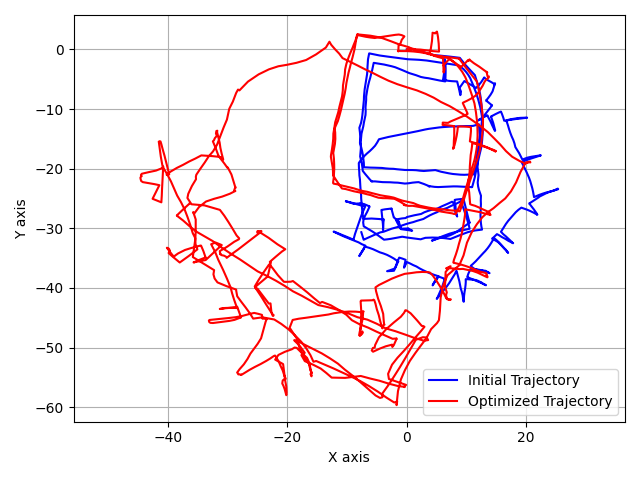
\includegraphics[width=0.6\columnwidth]{../figures/solve_pose_slam_2d_batch.png}}
        \caption{Batch Solution for 2D Pose SLAM on INTEL Dataset}
        \label{fig:2d_batch}
\end{figure}

Figure \ref{fig:2d_batch} shows the 2D pose SLAM result by the batch solution. It worth noting that the Gauss-Newton solver fell into a local minimum without perturbation and the optimization results are even worse than the initial trajectory.

\item \textbf{Incremental Solution:}

To solve a 2D pose SLAM problem incrementally, a modified version of the provided algorithm is proposed in Algorithm \ref{alg:incremental_2d}.
% TODO add error statistics

\begin{algorithm}[H]
    \caption{incremental\_solution (poses, edges)}\label{alg:incremental_2d}
    \begin{algorithmic}
    \Require $poses, edges$
    
    \State $priorNoiseModel \gets $ diagonal noise model
    \State $isam \gets ISAM2()$ \Comment Initialize iSAM2 solver with proper parameters
    \For {each $pose$ in $poses$}
        \State $graph \gets NonlinearFactorGraph()$
        \State $initialEstimate \gets Values()$
        \State $(id_p,\ currPose) \gets pose$
        \If {$id_p == 0$}
            \State $graph.add(PriorFactorPose(0, currPose, priorNoiseModel))$
            \State $initialEstimate.insert(id_p, currPose)$
        \Else 
            \State $prevPose \gets result.atPose(id_p - 1)$
            \State $initialEstimate.insert(id_p, currPose)$
            \For {each $edge$ in $edges$}
                \State $(id_{e1},\ id_{e2},\ poseBetween,\ infoVec) \gets edge$
                \If {$id_{e2} == id_p$}
                    \State $infoMat \gets constructInfoMat(infoVec)$
                    \State $noiseModel \gets noiseModel.Gaussian.Information(infoMat)$
                    \State $graph.add(BetweenFactorPose(id_{e1}, id_{e2}, poseBetween, noiseModel))$
                \EndIf
            \EndFor
        \EndIf
    \EndFor
    \State $isam.update(graph, initialEstimate)$ \Comment Perform incremental update to iSAM2's internal Bayes tree
    \State $result \gets isam.calculateEstimate()$
    
    \end{algorithmic}
\end{algorithm}

To reconstruct a information matrix from a list of its upper triangular entries
\begin{enumerate}
    \item Create a zero matrix $A$ with corresponding dimensions.
    \item Loop over and assign values to its upper triangular elements.
    \item Return $A + A.T - diag(A.diagonal)$
\end{enumerate}

To tune a iSAM2 solver
\begin{enumerate}[1.]
    \item $RelinearizeThreshold$ Only relinearize variables whose linear delta magnitude is greater than this threshold (default: 0.1).
    \item $MaxIterations$ Only relinearize any variables every relinearizeSkip calls to $ISAM2.update$  (default: 10).
\end{enumerate}

\begin{figure}[H]
    \centering
        \textsf{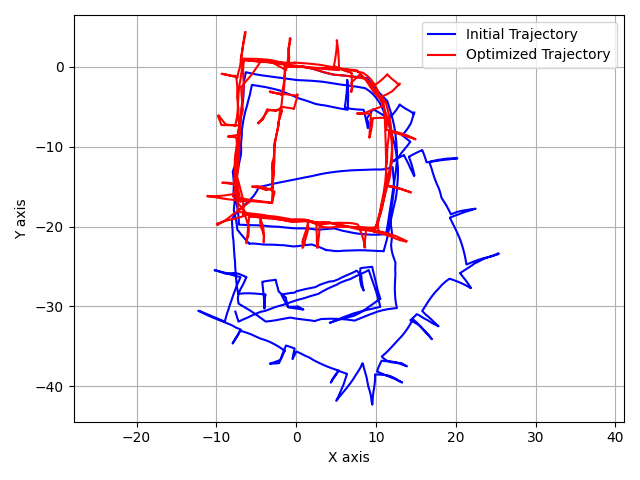
\includegraphics[width=0.6\columnwidth]{../figures/solve_pose_slam_2d_incremental.png}}
        \caption{Incremental Solution for 2D Pose SLAM on INTEL Dataset}
        \label{fig:solve_pose_slam_2d_incremental}
\end{figure}

Figure \ref{fig:solve_pose_slam_2d_incremental} shows the 2D pose SLAM result by the incremental solution.
% TODO add error statistics

\end{enumerate}




\section{3D Graph SLAM}\label{sec:3d}

\begin{enumerate}[A.]

\item This part is the same as Section \ref{sec:2d} A.

\item \textbf{Batch Solution:}

To solve a 3D pose SLAM problem in batch
\begin{enumerate}[1.]
    \item Construct a factor graph from data. A G2O file in this case, where edges are odometry measurements and verteies are initial guess of robot poses. Use $readG2o()$ will be fast and efficient.
    \item Add a prior to the pose having index zero. A diagonal noise model with zero mean and small variances can be chosen as a naive prior, a better way is using the first pose guess as the prior.
    \item Create the Gauss-Newton optimizer with proper parameters.
    \item Perform graph optimization and plot results.
\end{enumerate}

To tune a Gauss-Newton optimizer
\begin{enumerate}[1.]
    \item $Verbosity$ The printing verbosity during optimization (default SILENT), and set it to TERMINATION will show information about stopping conditions.
    \item $MaxIterations$ The maximum iterations to stop iterating (default 100).
    \item $RelativeErrorTol$ The maximum relative error decrease to stop iterating (default 1e-5).
\end{enumerate}

\begin{figure}[H]
    \centering
        \textsf{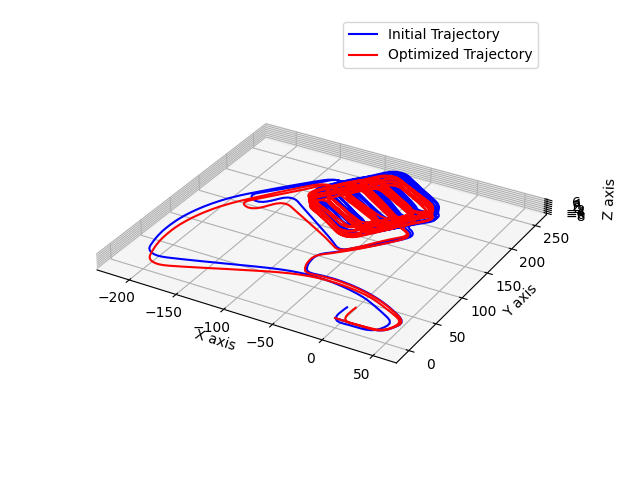
\includegraphics[width=0.65\columnwidth]{../figures/solve_pose_slam_3d_batch.png}}
        \caption{Batch Solution for 3D Pose SLAM on GARAGE Dataset}
        \label{fig:solve_pose_slam_3d_batch}
\end{figure}

Figure \ref{fig:solve_pose_slam_3d_batch} shows the 3D pose SLAM result by the batch solution. 
Two side views in X-Y plane and Y-Z plane of trajectories are plotted in Figure \ref{fig:solve_pose_slam_3d_batch_view}.
% TODO add error statistics

\begin{figure}[H]
    \centering
    \begin{subfigure}[b]{0.45\columnwidth}
        \centering
        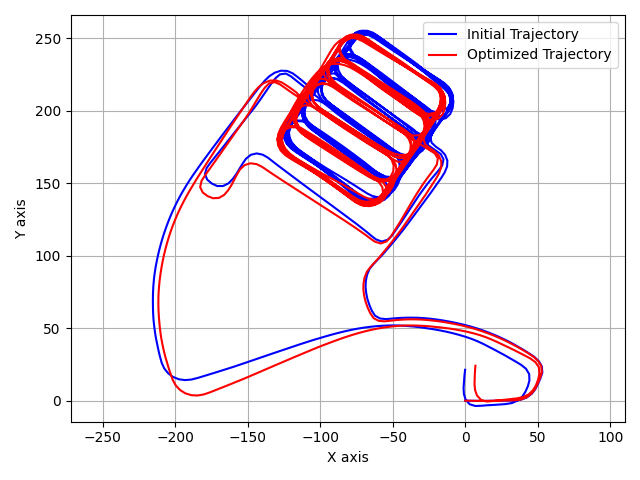
\includegraphics[width=\columnwidth]{../figures/solve_pose_slam_3d_batch_x_y.png}
        \caption{X-Y View}
        \label{fig:solve_pose_slam_3d_batch_x_y}
    \end{subfigure}
    \begin{subfigure}[b]{0.45\columnwidth}
        \centering
        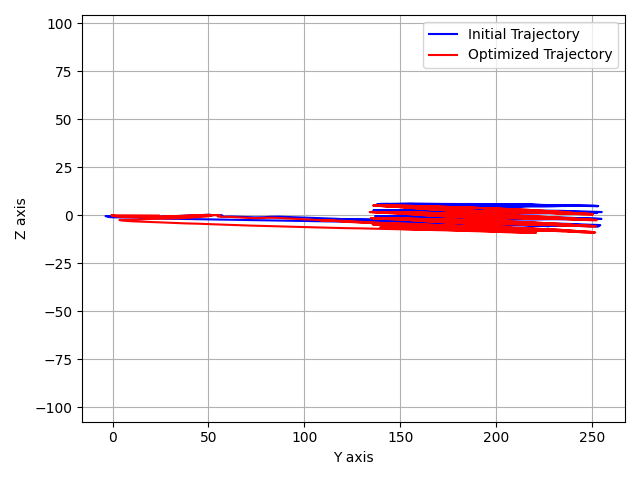
\includegraphics[width=\columnwidth]{../figures/solve_pose_slam_3d_batch_y_z.png}
        \caption{Y-Z View}
        \label{fig:solve_pose_slam_3d_batch_y_z}
    \end{subfigure}
    \caption{Side Views for 3D Batch Solution}
    \label{fig:solve_pose_slam_3d_batch_view}
\end{figure}

\item \textbf{Incremental Solution:}

To solve a 3D pose SLAM problem incrementally, a modified version of the provided algorithm is proposed in Algorithm \ref{alg:incremental_2d}.

To tune a iSAM2 solver
\begin{enumerate}[1.]
    \item $RelinearizeThreshold$ Only relinearize variables whose linear delta magnitude is greater than this threshold (default: 0.1).
    \item $MaxIterations$ Only relinearize any variables every relinearizeSkip calls to $ISAM2.update$  (default: 10).
\end{enumerate}

\begin{figure}[H]
    \centering
        \textsf{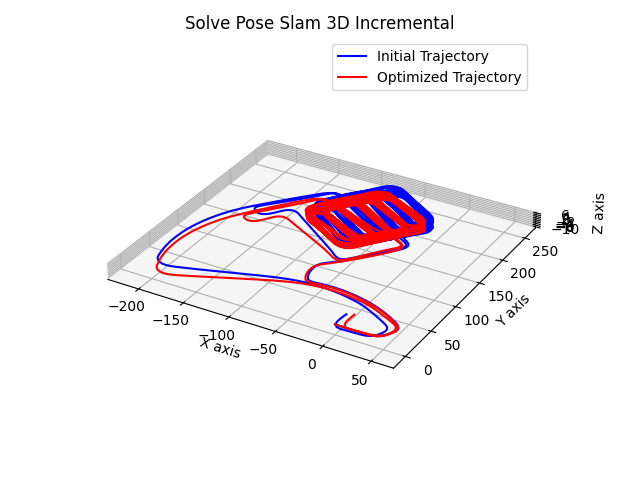
\includegraphics[width=0.65\columnwidth]{../figures/solve_pose_slam_3d_incremental.png}}
        \caption{Incremental Solution for 3D Pose SLAM on GARAGE Dataset}
        \label{fig:solve_pose_slam_3d_incremental}
\end{figure}

Figure \ref{fig:solve_pose_slam_3d_incremental} shows the 3D pose SLAM result by the incremental solution. 
Two side views in X-Y plane and Y-Z plane of trajectories are plotted in Figure \ref{fig:solve_pose_slam_3d_incremental_view}.
% TODO add error statistics

\begin{figure}[H]
    \centering
    \begin{subfigure}[b]{0.45\columnwidth}
        \centering
        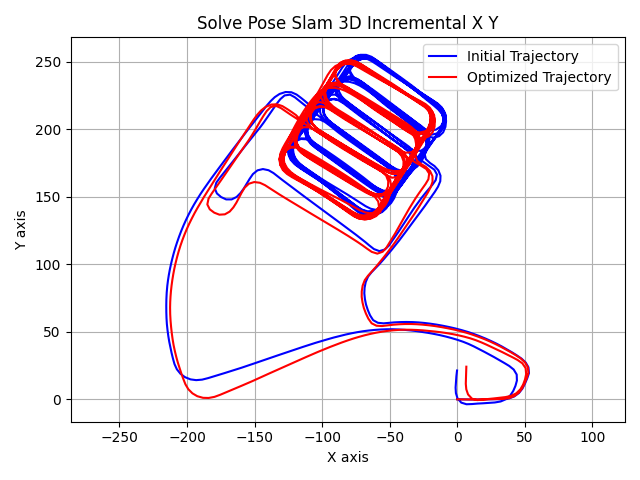
\includegraphics[width=\columnwidth]{../figures/solve_pose_slam_3d_incremental_x_y.png}
        \caption{X-Y View}
        \label{fig:solve_pose_slam_3d_incremental_x_y}
    \end{subfigure}
    \begin{subfigure}[b]{0.45\columnwidth}
        \centering
        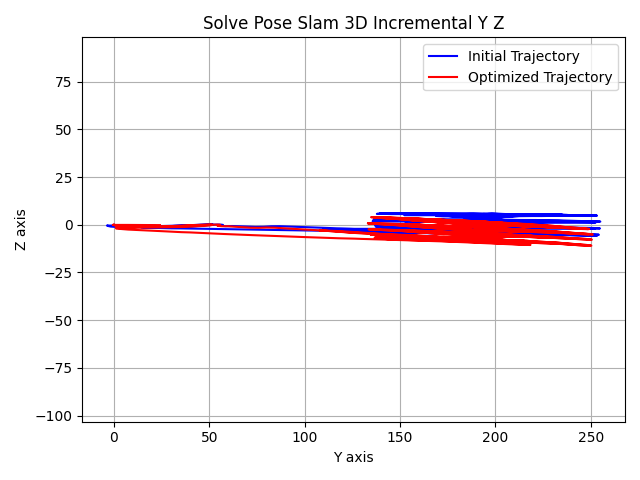
\includegraphics[width=\columnwidth]{../figures/solve_pose_slam_3d_incremental_y_z.png}
        \caption{Y-Z View}
        \label{fig:solve_pose_slam_3d_incremental_y_z}
    \end{subfigure}
    \caption{Side Views for 3D Incremental Solution}
    \label{fig:solve_pose_slam_3d_incremental_view}
\end{figure}


\end{enumerate}




\end{document}
